%\documentclass[10pt,preprint]{aastex}  % for e-submission to ApJ - one column
%\documentclass[12pt,preprint2]{aastex}  % for e-submission to ApJ - two column

\documentclass[iop,apjl, twocolappendix]{emulateapj}   % makes it look like the ApJ format

\pdfoutput=1

\usepackage{graphicx}
\usepackage{epsfig}
\usepackage{amsmath}
\usepackage{subfigure} 
%\usepackage{subcaption} 
\usepackage{comment}
\usepackage{hyperref}
\usepackage{amssymb}
\usepackage{apjfonts}
\usepackage{amsmath}
\usepackage{latexsym}
\usepackage{color}
\usepackage{algorithm}
\usepackage{algpseudocode}
\usepackage[usenames,dvipsnames,svgnames,table]{xcolor}
\usepackage{hyperref}
\usepackage[all]{hypcap}    %for going to the top of an image when a figure reference is clicked
\hypersetup{
	colorlinks,
		citecolor=blue,
		filecolor=blue,
		linkcolor=blue,
		urlcolor=blue
	}
\makeatletter
\algrenewcommand\ALG@beginalgorithmic{\ttfamily}
\makeatother

\newcommand{\red}[1]{\textcolor{red}{#1}}
\newcommand{\blue}[1]{\textcolor{blue}{#1}}
\newcommand{\green}[1]{\textcolor{green}{#1}}

\shorttitle{AGN Thermal Heating} 
\shortauthors{F. glines et al.}

\begin{document}\title{Active Galactic Nuclei Thermal Heating}

\author{
  Forrest W. Glines \altaffilmark{1,2,3}, Brian W. O'Shea \altaffilmark{1,2}, G. Mark Voit\altaffilmark{1}
}

\affil{$^{1}${Department of Physics and Astronomy,
    Michigan State University, East Lansing, MI 48824, USA} }
\affil{$^{2}${Department of Compuational Mathematics, Science and Engineering,
    Michigan State University, East Lansing, MI 48824, USA} }
\affil{$^{3}${\href{mailto:glinesfo@msu.edu}{glinesfo@msu.edu}}}

\label{firstpage}

\begin{abstract}
\end{abstract}

\keywords{}

\section{Introduction}
\label{sec:introduction}


\textbullet Cool-core problem and current resolution?

\textbullet Elaborate on Voit analytical work - the toy model - a heating curve balancing
cooling that preserves the entropy profile

\textbullet Elaborate on Greg's work?

\textbullet AGN feedback in other simualtions

\textbullet Paper outline

Galaxy clusters have predictable entropy profiles whose shape (although not
necessarily normalization) are mass-independent.
\cite{cavagnolo_intracluster_2009} Although -ray observations of the
intracluster medium (ICM) indicate that the central cooling times  in some
galaxy clusters are much shorter than the age of the universe, no cooling
catastrophe is observed. This argues that there is a heating mechanism that
offsets the cooling and acts on timescales comparable to the cooling time.
Given a variety of physical considerations, the primary heating source is
largely accepted to be active galactic nuclei (AGN).  What is not
well-understood, however, is the manner in which AGN deposit energy into the
ICM.   \textbf{The goal of this work} is to constrain the radial dependence of
the AGN energy injection by comparing a simplified model of AGN heating with
key X-ray observable quantities. This effort builds on work by Meece et. al.
\cite{meece_jr_agn_2016,meece_triggering_2017} using an idealized model of
thermal feedback over the cluster core following a power law, inspired by
analytical work by Voit et. al.
\cite{voit_global_2017}.

\section{Methodology}
\label{sec:methodology}

\subsection{AGN Feedback}
\textbullet Energy from the AGN is deposited as purely thermal energy in a sphere
encompassing the cluster.

\begin{equation}
	\dot{e}(r) = \left( \frac{r}{r_c} \right )^{-\alpha} \exp { -r/r_c}
\end{equation}

\textbullet Details of feedback: smoothing length, cut off radius, scaling factor

Using a cutoff radius $r_c= 1\text{ Mpc}.$ In order to avoid the asymptote at
the origin, the radius $r$ is smoothed to a minimum radius of $1\text{ kpc}$
The total AGN heat tracks the cooling rate, which is updated every $10
\text{Myr}$ We use a different $\alpha$ for each run, sampling from $2.0$ to
$2.9$ in $0.1$ increments and $2.5$ to $2.7$ in $0.05$ increments.

\textbullet Conic feedback
\begin{equation}
	\dot{e}(\theta) \propto \cos^2 \theta 
\end{equation}
where $\theta$ is the polar angle.

\textbullet Each simulation is run for $8 \text{Gyr}$, or appoximately $4$ sound crossing
times for the cluster. 


Energy from AGN feedback is deposited thermally in a sphere encompassing the
cluster. The deposited energy follows a power law:
\vspace{-0.5em}
\begin{equation}
	\dot{e}(r) \propto \left( \frac{r}{r_c} \right )^{-\alpha} \text{ erg} \text{ s}^{-1} \text{ cm}^{-3}.
	\vspace{-0.5em}
\end{equation}

\noindent
The thermal energy deposited in the cluster is scaled to exactly offset the
total cooling within the cluster, thus maintaining overall energy balance.
Simulations were run with a range of radial heating distributions ranging from
$\alpha = 2.0$ to 2.9. 
All simulations used the adaptive mesh code \texttt{Enzo} \cite{bryan_enzo:_2014} using AGN feedback algorithms modified from
\cite{meece_jr_agn_2016,meece_triggering_2017}.

\subsection{Initial Conditions}
\label{sec:initial_conditions}
Simulations are initialized in a Perseus-like configuration, in the manner
of Meece \cite{meece_triggering_2017} and Li et al.\ \cite{li_cooling_2015} 

\section{Results}

\textbullet Feedback failed to self regulate

\textbullet Core entropy increases with $\alpha$

\textbullet Surface brightness decreases with $\alpha$

\textbullet <More results from conic feedback>

\label{sec:results}
\begin{figure}
	\begin{center}
		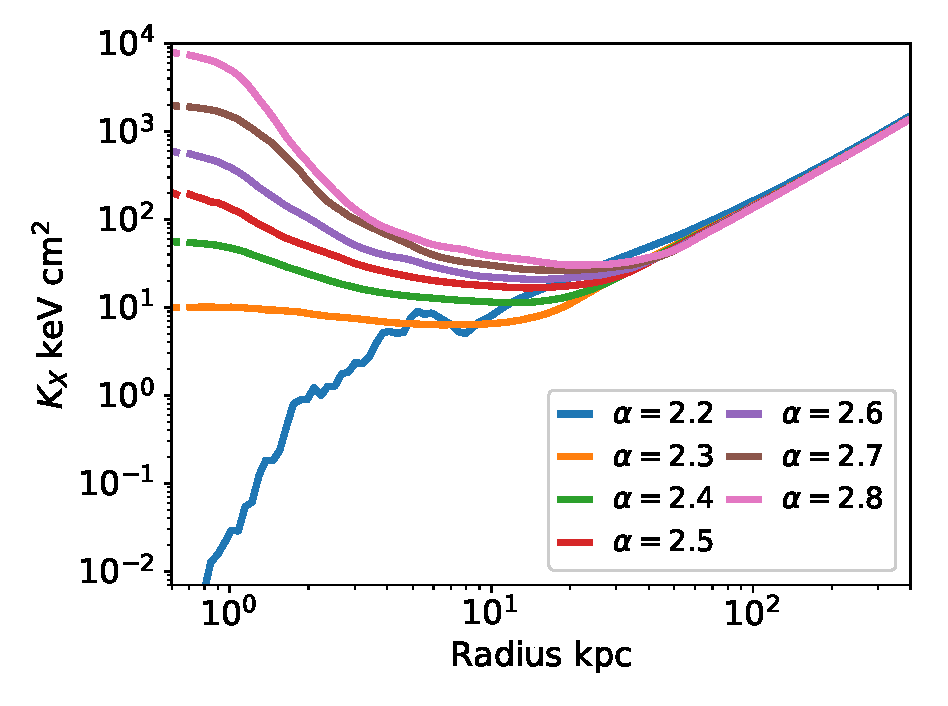
\includegraphics[width=0.49\linewidth]{figures/entropyVradius.eps}
		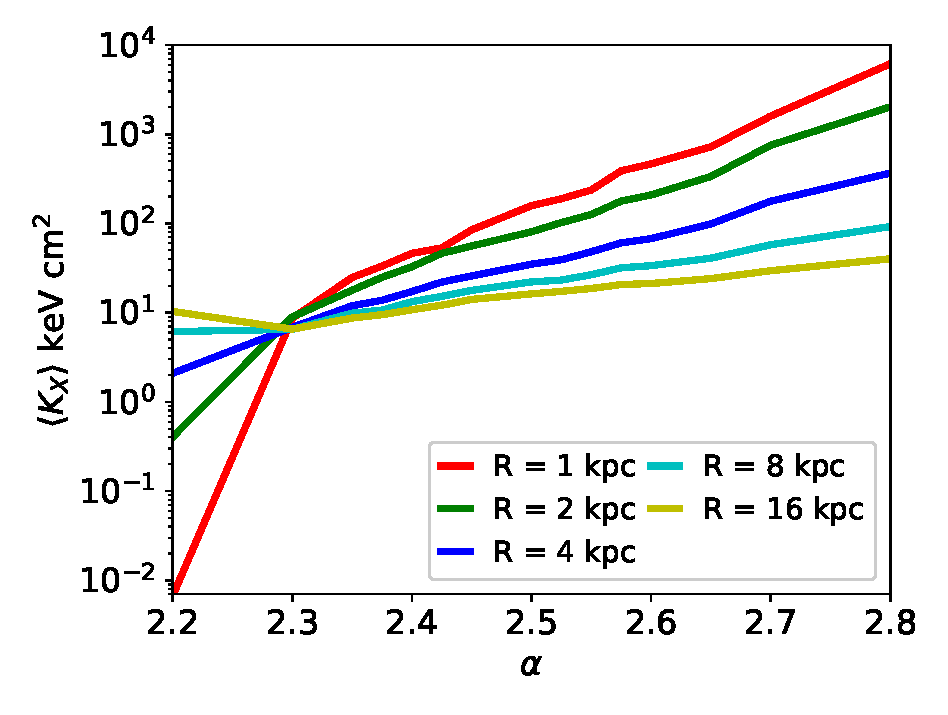
\includegraphics[width=0.49\linewidth]{figures/entropyValpha.eps}
	\end{center}
	\caption{
		\textbf{Left:}  Mean entropy as a function of spherical radius from
	several representative simulations.  \textbf{Right:} Mean cluster core
	entropy calculated within impact parameters ranging from $R = 2^0 - 2^4$ proper
	kpc for the same set of simulations, as a function of $\alpha$.  In both
	panels, entropy is calculated by the mass-weighted temperature and the
	volume-weighted density, and all data is taken after 700 Myr of simulation
	evolution.}
\end{figure}

\begin{figure}
	\begin{center}
		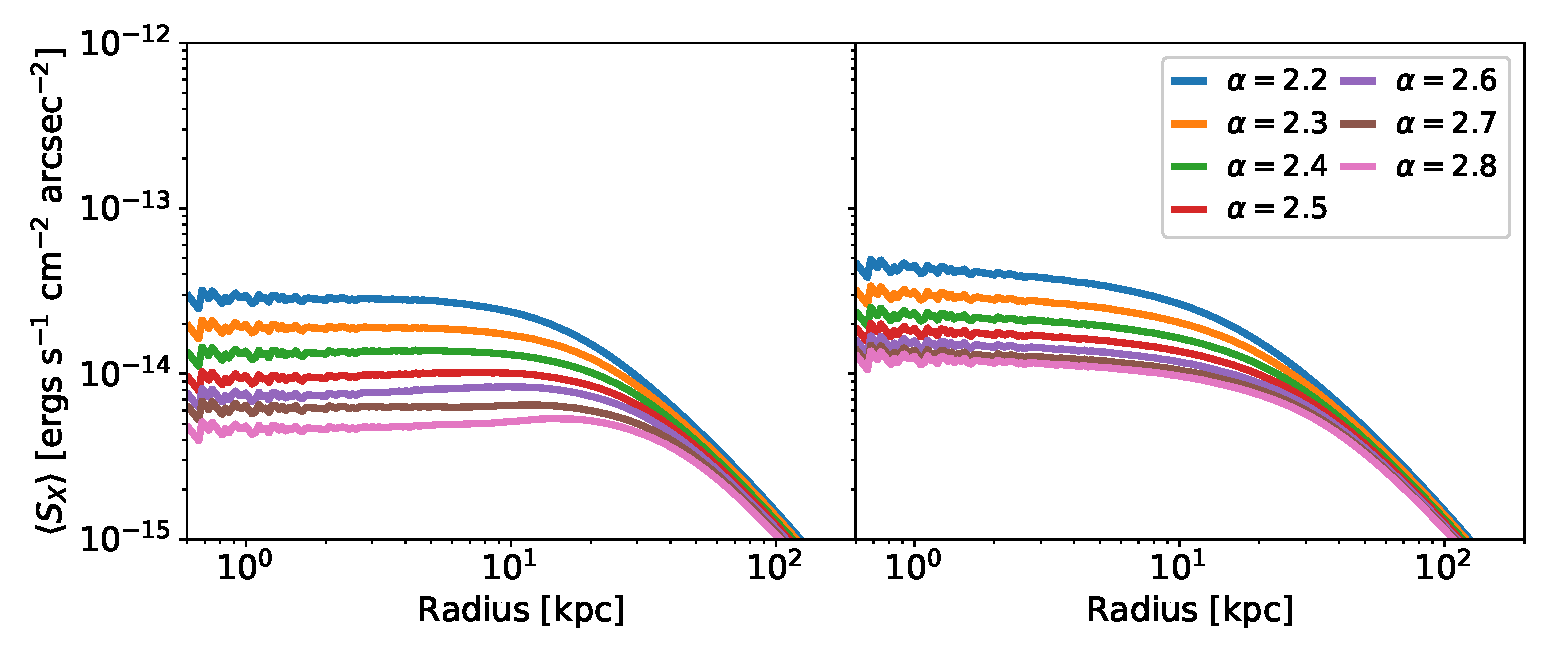
\includegraphics[width=0.49\linewidth]{figures/surfaceBrightnessVradius.eps}
		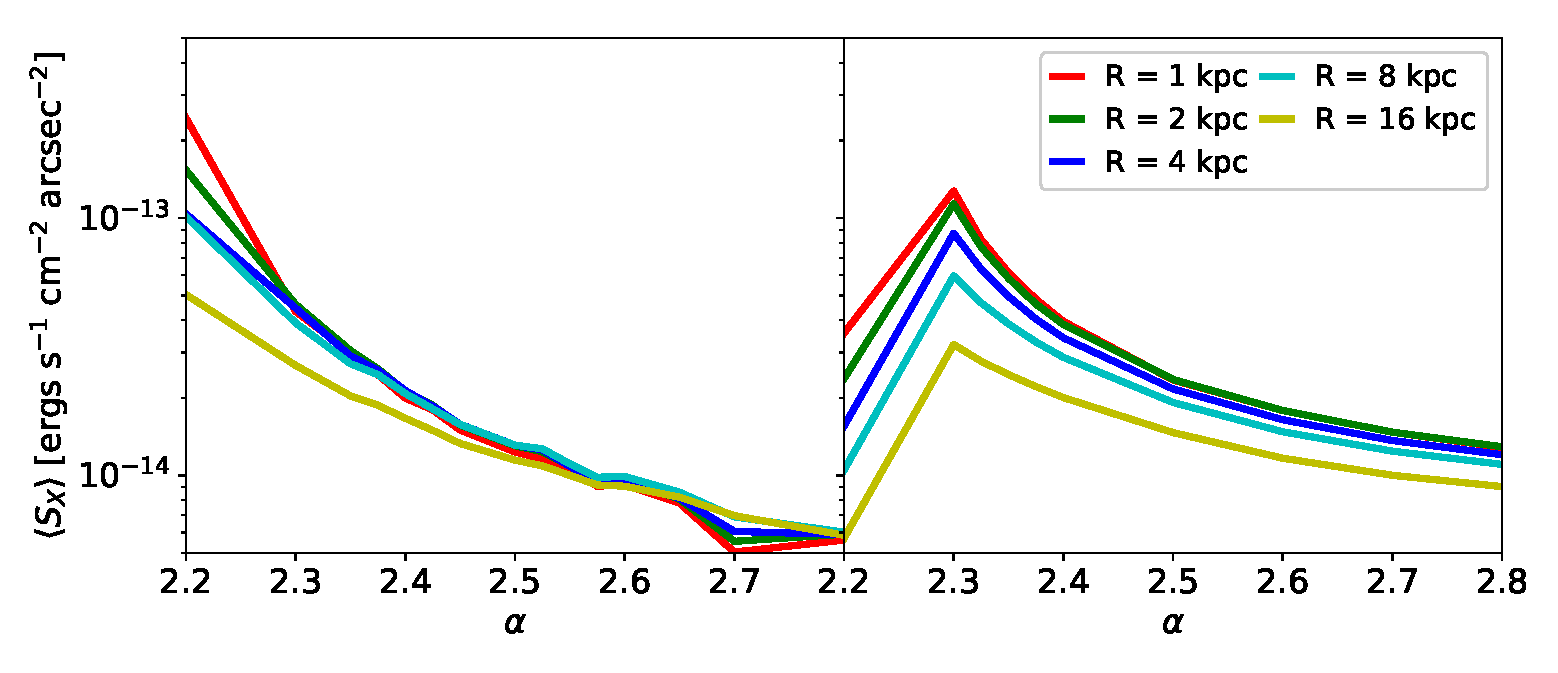
\includegraphics[width=0.49\linewidth]{figures/surfaceBrightnessValpha.eps}
	\end{center}
	\caption{
		\textbf{Left:} Mean simulated X-ray surface brightness in the $0.5
	-2.0 \text{ keV}$ band as a function of observing radius. \textbf{Right:}
	Mean surface brightness of cores of radii $R = 2^0 - 2^4$ proper kpc from
	the same simulations as a function of $\alpha$. All data is taken after 700
	Myr of simulation evolution.
	%However, lower $\alpha$ simulations progress to cooling catastrophe
	%sooner. Here the $\alpha=2.2$ simulation is going through a collapse.
}
\end{figure}

\begin{figure}
	\begin{center}
		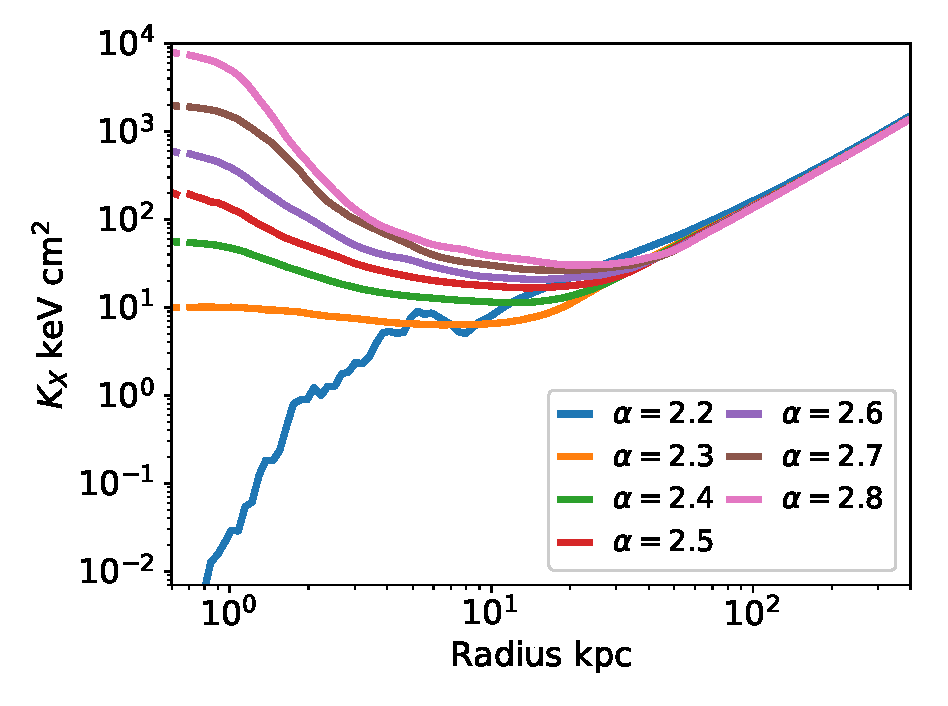
\includegraphics[width=0.49\linewidth]{figures/entropyVradius.eps}
		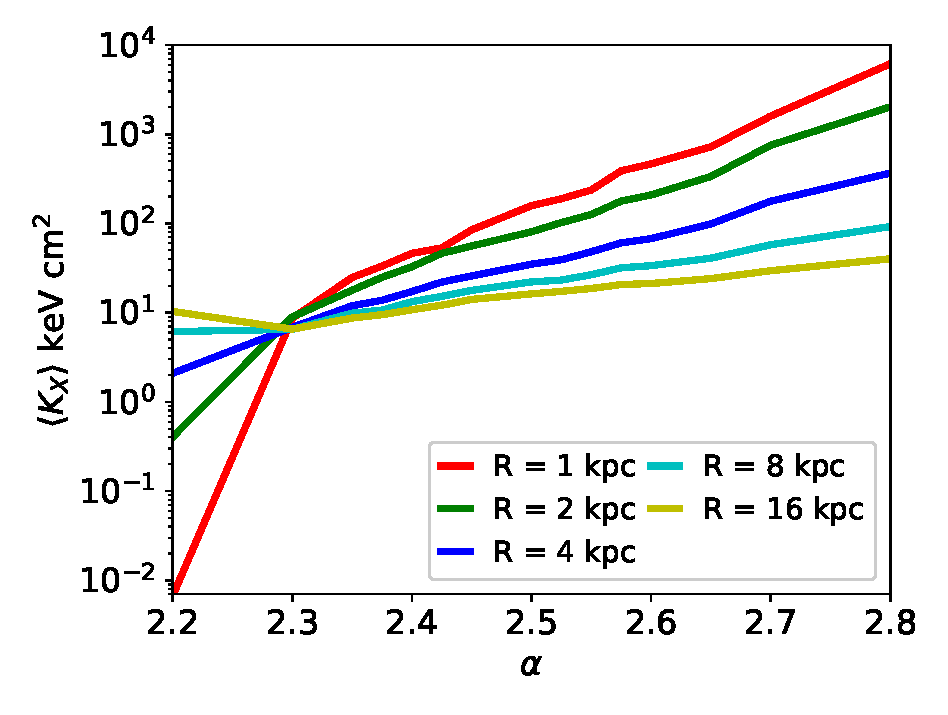
\includegraphics[width=0.49\linewidth]{figures/entropyValpha.eps}
	\end{center}
	\caption{
		\textbf{Left:}  Mean entropy as a function of spherical radius from
	several representative simulations.  \textbf{Right:} Mean cluster core
	entropy calculated within impact parameters ranging from $R = 2^0 - 2^4$ proper
	kpc for the same set of simulations, as a function of $\alpha$.  In both
	panels, entropy is calculated by the mass-weighted temperature and the
	volume-weighted density, and all data is taken after 700 Myr of simulation
	evolution.}
\end{figure}

\begin{figure}
  \begin{center}
    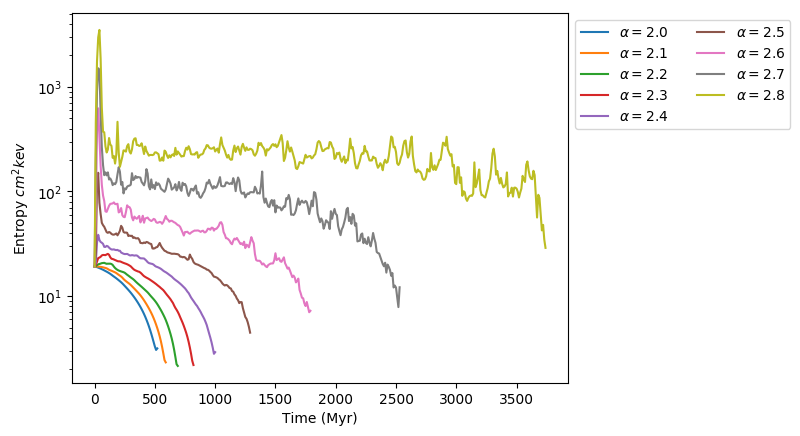
\includegraphics[width=0.9\linewidth]{figures/core_vw_entropy.png}
  \end{center}
  \caption{Mean core entropy on the inner $10 \text{ kpc}$ as
  a function of time from several representative simulations.  evolution.}
\end{figure}

\begin{figure}
  \caption{Cold gas fraction as a function of time}
\end{figure}



\section{Discussion}
\label{sec:discussion}

\textbullet Higher energy input into core leads to slower collapse times, larger flat entropy cores.

\textbullet Formation of multiphase gas leads to collapse?

Higher $\alpha$, corresponding to more energy input at the cluster core,
predictably raised core entropy. Lower $\alpha$ left a flat entropy
profiles closer to the initial conditions.  The higher $\alpha$
simulations push out enough gas from the core to decrease x-ray
brightness. 

Although this is a very simplified model of cluster feedback, it can be used to
constrain the broad properties of AGN feedback -- in particular, the radial
dependence of its heat deposition -- using X-ray observations.  In the near
future, we will make direct comparisons to Chandra X-ray data of entropy and
surface brightness profiles  using the ACCEPT survey
\cite{cavagnolo_intracluster_2009} and its successors.

\acknowledgments
\section{Acknowledgments}
\label{sec:acknowledgments}
This project has been supported by NASA through Astrophysics Theory Program
grant \#NNX15AP39G and Hubble Theory Grant HST-AR-13261.01-A, and by the
NSF through grant AST-1514700.  The simulations were run on the NASA
Pleiades supercomputer through allocation SMD-16-7720.  \texttt{Enzo} and
\texttt{yt} are developed by a large number of independent researchers from
numerous institutions around the world. Their commitment to open science
has helped make this work possible.

%\input{apj-bib}
\bibliographystyle{apj}

\bibliography{apj-jour,AGNThermal2018}

\end{document}
